










\subsection*{\hspace*{\parindent}Задание 3} 
Для двух выборок, приведенных в задании~1, найти выборочные средние, 
выборочные дисперсии и средние квадратичные отклонения, выборочный 
коэффициент корреляции, написать уравнения выборочных прямых 
регрессии и построить их.

\par
{\em Решение.}
Простейшей характеристикой распределения является выборочное среднее, 
которое для простой статистической совокупности объема $ n $ вычисляется 
по формуле:

$$  
  \bar{x} = \frac{1}{n} \sum_{i=1}^n x_i{,}\ \text{где } x_i \text{~--- очередной 
  элемент выборки.}
$$

Выборочное среднее является приближенной оценкой математического ожидания 
изучаемой случайной величины. Для характеристики разброса значений случайной 
величины относительно ее среднего значения используются выборочная дисперсия 
$ S^2 $, являющаяся оценкой теоритической дисперсии. Для простой совокупности 
выборочная дисперсия вычисляется по формуле:

$$  
	S^2 = \frac{1}{n} \sum_{i=1}^n {(x_i - \bar{x})} = \overline{(x - \bar{x})^2}. 
$$

Выборочное среднеквадратичное отклонение $ S = \sqrt{S^2} $ является 
оценкой теоретического среднеквадратического отклонения $ \sigma $.

На практике значение $ S^2 $ вычисляется по более простой формуле:

$$  
	S^2 = \frac{1}{n} \sum_{i=1}^n {(x_i^2 - \bar{x}^2)} = \overline{x^2} - 
	\bar{x}^2.
$$

Если объем выборки невелик, то $ S^2 $  является смещенной оценкой 
теоритической дисперсии: $ M(S^2) \neq D(\xi)$. Чтобы получить несмещенную 
оценку, вводят поправочный коэффициент $ \frac{n}{n-1} $ и получают так 
называемую исправленную поправочную дисперсию 

$$  
	S^{*2} = \frac{n}{n-1} S^2 = \frac{1}{n-1} \sum_{i=1}^n {(x_i - \bar{x})} = 
	\frac{\sum\limits_{i=1}^k {x_i^2 - n \bar{x}^2}}{n-1}. 
$$

Вычислим требуемые параметры для обеих выборок по формулам для простой 
совокупности и для данных, сгруппированных при построения гистограммы 
в задании~1. Результаты привидены в табл.~\ref{tab:7}.

\begin{table}[h]
\caption{Точечные оценки параметров распределения для выборок 1 и 2.}\label{tab:7}
\begin{tabular}{|c|c|c|c|c|c|c|}
\hline
 &  $ \bar{x} $ & $ S^2 $ & $ S $  & $ S^{*2} $ & $ S^* $ \\
\hline
Выборка 1  &  
-1{,}830271    & 
4{,}247264      & 
2{,}060889       & 
4{,}424233 & 
2{,}103386 
\\  
\hline
Выборка 2  & 
1{,}967553    & 
3{,}462236      & 
1{,}860708       & 
3{,}606495 & 
1{,}899078 
\\
\hline
\end{tabular}
\end{table}


Далее вычисляется выборочной коэффициент корреляции и строятся выборочные прямые регрессии. Вместо теоритического коэффициента корреляции и теоритических среднеквадратических отклонений вычисляются выборочные их оценки по данным выборки случайной величины 
$ (\xi;\zeta) $ объема $ n $.

Вначале строится корреляционная таблица, каждая $ i $-я строка таблицы соответствует значению $ \xi_i $, а каждый $ j $-й столбец --- значению $ \zeta_i $. На пересечении строки $ i $ и столбца $ j $ записывается число, показывающее, сколько раз в выборке встретилась пора $ (\xi_i;\zeta_j) $.
Если таких пар нет, клетка остается пустой. При обработке
корреляционной таблицы в последнем столбце указывают сумму частот по строкам, а в последней строке --- сумму частот по столбцам. Структура корреляционной таблицы представлена в талице~\ref{tab:8}.

\begin{table}
\caption{Структура корреляционной таблицы.}\label{tab:8}
\begin{center}
\begin{tabular}{|c|c|c|c|c|c|}
\hline
 \backslashbox{\parbox[c][1.5em][c]{3em}{$\xi$}}{$\zeta$} &  $ y_1 $  &   $ y_2 $ & $ \cdots $ & $ y_s $  & $ n_{i \bullet} = \sum\limits_{j=1}^s n_{ij} $  \\
\hline
$ x_1 $ &  $n_{11}$  & $n_{12}$ & $\cdots$ & $n_{1s}$ & $n_{1 \bullet }$  \\  
\hline
$ x_2 $ &  $n_{21}$  & $n_{22}$ & $\cdots$ & $n_{2s}$ & $n_{2 \bullet }$  \\  
\hline
$ \vdots $ &  $ \vdots $ & $ \vdots $ & $ \ddots $ & $ \vdots $ &  $ \vdots $  \\  
\hline
$ x_k $ &  $n_{k1}$  & $n_{k2}$ & $\cdots$ & $n_{ks}$ & $n_{k \bullet }$  \\  
\hline
$ n_{\bullet j} = \sum\limits_{i=1}^k n_{ij} $  &  $n_{ \bullet 1}$  & $n_{ \bullet 2}$ & $\cdots$ & $n_{\bullet s}$ & 
 $\sum\limits_{i=1}^k{\sum\limits_{j=1}^s n_{ij}} $ \\ 
 \hline
\end{tabular}
\end{center}
\end{table}

Первый и последний столбцы корреляционной таблицы образуют статистическое распределение выборки случайной величины $ \xi $, а первая и последняя строки образуют выборку случайной величины $ \zeta $. Выборочные числовые характеристики по этим данным вычисляются по следующим формулам:

$$  
	\bar{x} = \frac{\sum\limits_{i=1}^k {n_{i \bullet} x_i}}{n} \text{, } 
	S_x^{*2} = \frac{\sum\limits_{i=1}^k {n_{i \bullet} x_i^2 - n \bar{x}^2}}{n}{, } 
$$
$$  
	\bar{y} = \frac{\sum\limits_{i=1}^k {n_{\bullet j} y_i}}{n} \text{, } 
	S_y^{*2} = \frac{\sum\limits_{i=1}^k {n_{\bullet j} y_i^2 - n \bar{y}^2}}{n}{.} 
$$

Далее вычисляется выборочный коэффициент корреляции  $ r^{*}_{xy} $, являющийся статистической оценкой теоретического коэффициента корреляции:
$$  
	r^{*}_{xy}  = \frac{\overline{xy} - \bar{x}\bar{y}}{S^*_x S^*_y} \text{, где } 
	\overline{xy} = \frac{\sum\limits_{i=1}^k{\sum\limits_{j=1}^s {n_{ij} x_i y_j}}}{n}{. } 
$$

Выборочные уравнения прямых регрессии $ \zeta $ на $ \xi $ и $ \xi $ на $ \zeta $ имеют вид:
$$  
	y = r^{*}_{xy} \frac{S^*_y}{S_x^*}(x - \bar{x}) + \bar{y} \text{  (уравнение прямой регрессии~}  \zeta \text{ на } \xi){,}
$$
$$  
	x= r^{*}_{xy} \frac{S^*_x}{S_y^*}(y - \bar{y}) + \bar{x}  \text{  (уравнение прямой регрессии~} \xi \text{ на } \zeta ){.}
$$

Они задают линейную зависимость условных выборочных математических ожиданий (вернее, условных средних) одной случайной величины (левые части уравнений) от значения другой случайной величины ($ x\ \text{или}\ y\ $ в правых частях уравнений).

В предположении что $ i $-е значения выборок образуют $ i $-ю пару  $ (\xi_i;\zeta_i) $ $ (1 \leqslant i \leqslant 25) $, составим корреляционную таблицу (табл.~\ref{tab:9}). Также схематически изобразим выборку 
случайной величины $(\xi;\zeta)$, отметив пары $(x_i, y_i)$ на плоскости $Oxy$ (рис.~\ref{pic:11})





  

  

  

  

  

  

  

  

  

  

  

  

  

  

  

  

  

  

  

  

  

  

  

  

  


\newpage



\begin{table}[h]
\begin{tabular}{|>{\tiny}c||>{\tiny}c|>{\tiny}c|>{\tiny}c|>{\tiny}c|>{\tiny}c|>{\tiny}c|>{\tiny}c|>{\tiny}c|>{\tiny}c|>{\tiny}c|>{\tiny}c|>{\tiny}c|>{\tiny}c|>{\tiny}c|>{\tiny}c|>{\tiny}c|>{\tiny}c|>{\tiny}c|>{\tiny}c|>{\tiny}c|>{\tiny}c|>{\tiny}c|>{\tiny}c|>{\tiny}c|>{\tiny}c||>{\tiny}c|}
\hline
\raisebox{5mm}{$\xi\setminus\zeta$} & \rotatebox{90}{$0{,}160135$} & \rotatebox{90}{$0{,}196073$} & \rotatebox{90}{$0{,}306291$} & \rotatebox{90}{$0{,}353165$} & \rotatebox{90}{$0{,}36036$} & \rotatebox{90}{$0{,}423245$} & \rotatebox{90}{$0{,}591799$} & \rotatebox{90}{$0{,}82157$} & \rotatebox{90}{$0{,}884235$} & \rotatebox{90}{$0{,}900104$} & \rotatebox{90}{$1{,}063247$} & \rotatebox{90}{$1{,}093911$} & \rotatebox{90}{$1{,}157221$} & \rotatebox{90}{$1{,}30273$} & \rotatebox{90}{$1{,}565542$} & \rotatebox{90}{$1{,}600444$} & \rotatebox{90}{$2{,}341499$} & \rotatebox{90}{$2{,}548808$} & \rotatebox{90}{$3{,}137087$} & \rotatebox{90}{$3{,}442844$} & \rotatebox{90}{$3{,}518885$} & \rotatebox{90}{$4{,}209723$} & \rotatebox{90}{$4{,}51201$} & \rotatebox{90}{$4{,}768065$} & \rotatebox{90}{$7{,}929842$} & \raisebox{5mm}{$n_{i\bullet}$} \\
\hhline{|=::=========================::=|}

-5{,}581626 &  &  &  &  &  &  &  &  &  &  &  &  &  &  &  &  &  &  &  &  &  &  & $1$ &  &  & $1$ \\ \hhline{-||-------------------------||-}

-4{,}46825 &  &  &  &  &  &  &  &  &  &  &  &  &  &  &  & $1$ &  &  &  &  &  &  &  &  &  & $1$ \\ \hhline{-||-------------------------||-}

-4{,}440732 &  & $1$ &  &  &  &  &  &  &  &  &  &  &  &  &  &  &  &  &  &  &  &  &  &  &  & $1$ \\ \hhline{-||-------------------------||-}

-4{,}283991 &  &  &  &  &  &  &  &  &  & $1$ &  &  &  &  &  &  &  &  &  &  &  &  &  &  &  & $1$ \\ \hhline{-||-------------------------||-}

-3{,}719059 &  &  &  &  &  &  &  &  &  &  &  &  &  &  & $1$ &  &  &  &  &  &  &  &  &  &  & $1$ \\ \hhline{-||-------------------------||-}

-3{,}666468 &  &  &  &  &  &  &  &  &  &  &  &  &  &  &  &  &  &  &  &  &  & $1$ &  &  &  & $1$ \\ \hhline{-||-------------------------||-}

-3{,}621161 &  &  &  &  &  &  &  &  &  &  &  &  &  &  &  &  &  &  &  &  &  &  &  &  & $1$ & $1$ \\ \hhline{-||-------------------------||-}

-3{,}513652 &  &  & $1$ &  &  &  &  &  &  &  &  &  &  &  &  &  &  &  &  &  &  &  &  &  &  & $1$ \\ \hhline{-||-------------------------||-}

-3{,}443457 &  &  &  &  &  &  &  &  &  &  &  &  &  & $1$ &  &  &  &  &  &  &  &  &  &  &  & $1$ \\ \hhline{-||-------------------------||-}

-2{,}970003 &  &  &  &  &  &  &  &  &  &  &  &  &  &  &  &  &  & $1$ &  &  &  &  &  &  &  & $1$ \\ \hhline{-||-------------------------||-}

-2{,}801433 &  &  &  &  &  &  &  &  &  &  &  &  &  &  &  &  &  &  &  &  &  &  &  & $1$ &  & $1$ \\ \hhline{-||-------------------------||-}

-2{,}530841 &  &  &  &  &  &  &  &  & $1$ &  &  &  &  &  &  &  &  &  &  &  &  &  &  &  &  & $1$ \\ \hhline{-||-------------------------||-}

-2{,}251157 &  &  &  &  &  &  &  &  &  &  &  &  &  &  &  &  & $1$ &  &  &  &  &  &  &  &  & $1$ \\ \hhline{-||-------------------------||-}

-0{,}875469 &  &  &  &  &  &  &  &  &  &  &  &  &  &  &  &  &  &  &  & $1$ &  &  &  &  &  & $1$ \\ \hhline{-||-------------------------||-}

-0{,}745084 & $1$ &  &  &  &  &  &  &  &  &  &  &  &  &  &  &  &  &  &  &  &  &  &  &  &  & $1$ \\ \hhline{-||-------------------------||-}

-0{,}62873 &  &  &  &  &  &  &  &  &  &  &  & $1$ &  &  &  &  &  &  &  &  &  &  &  &  &  & $1$ \\ \hhline{-||-------------------------||-}

-0{,}546616 &  &  &  &  &  &  &  & $1$ &  &  &  &  &  &  &  &  &  &  &  &  &  &  &  &  &  & $1$ \\ \hhline{-||-------------------------||-}

-0{,}438544 &  &  &  &  &  &  &  &  &  &  & $1$ &  &  &  &  &  &  &  &  &  &  &  &  &  &  & $1$ \\ \hhline{-||-------------------------||-}

-0{,}111441 &  &  &  &  &  &  &  &  &  &  &  &  &  &  &  &  &  &  &  &  & $1$ &  &  &  &  & $1$ \\ \hhline{-||-------------------------||-}

-0{,}078647 &  &  &  &  &  & $1$ &  &  &  &  &  &  &  &  &  &  &  &  &  &  &  &  &  &  &  & $1$ \\ \hhline{-||-------------------------||-}

0{,}252497 &  &  &  &  &  &  &  &  &  &  &  &  &  &  &  &  &  &  & $1$ &  &  &  &  &  &  & $1$ \\ \hhline{-||-------------------------||-}

0{,}932521 &  &  &  & $1$ &  &  &  &  &  &  &  &  &  &  &  &  &  &  &  &  &  &  &  &  &  & $1$ \\ \hhline{-||-------------------------||-}

1{,}00652 &  &  &  &  & $1$ &  &  &  &  &  &  &  &  &  &  &  &  &  &  &  &  &  &  &  &  & $1$ \\ \hhline{-||-------------------------||-}

1{,}374713 &  &  &  &  &  &  & $1$ &  &  &  &  &  &  &  &  &  &  &  &  &  &  &  &  &  &  & $1$ \\ \hhline{-||-------------------------||-}

1{,}393335 &  &  &  &  &  &  &  &  &  &  &  &  & $1$ &  &  &  &  &  &  &  &  &  &  &  &  & $1$ \\ 

\hhline{|=::=========================::=|}
$n_{\bullet j}$ & $1$ & $1$ & $1$ & $1$ & $1$ & $1$ & $1$ & $1$ & $1$ & $1$ & $1$ & $1$ & $1$ & $1$ & $1$ & $1$ & $1$ & $1$ & $1$ & $1$ & $1$ & $1$ & $1$ & $1$ & $1$ & $25$ \\ \hline
\end{tabular}
\caption{Корреляционная таблица выборок 1 и 2, $x_i$ соответствуют упорядоченным значениям из выборки 1, 
а $y_j$~--- упорядоченным значениям из выборки 2, приведенным в табл.~\ref{tab:2}.}
\label{tab:7}
\end{table}
\newpage

\begin{figure}[h]
  \includegraphics[scale=1]{images/st.11.eps}
  \caption{Выборка случайной величины $(\xi;\zeta)$.}\label{pic:11}
\end{figure}




Коэффициент корреляции $ r^{*}_{xy} = -0{,}323006 $.

Уравнения прямых регрессии:


$$  
	y_x = -0{,}2916 x + 1{,}4338 \text{,}
$$


$$
	x_y = -0{,}3578 y  -1{,}1264 \text{.}
$$

Графики прямых регрессии изображены на рисунке~\ref{pic:12}.
\begin{figure}[h]
  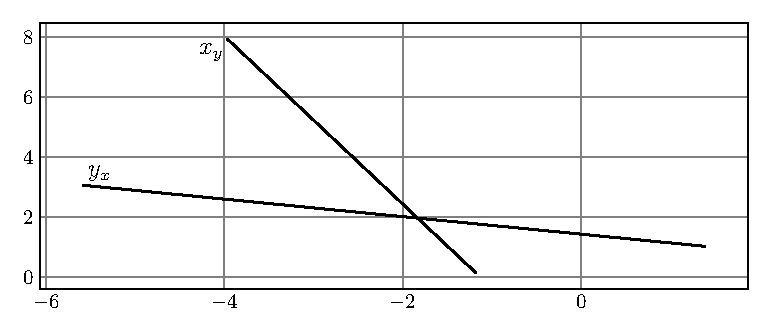
\includegraphics[scale=1]{images/st.12.eps}
  \caption{Графики прямых регрессии.}\label{pic:12}
\end{figure}
\endinput

